% *****************************************************************************
%
%        FASThesis Manual
%        (FASThesis Class File Documentation)
%
%        Faculty of Applied Sciences
%        University of West Bohemia
%
%        Manual & Explanatory Document
%        Copyright (c) 2022-2024 Kamil Ekštein, Dept. of Computer Science
%        and Engineering, Faculty of Applied Sciences, UWB
%
%        Version:  0.96
%		 Encoding: UTF-8
%		 TeXer:    pdflatex
%
%        Last modification on 11-Apr-2024 by KE
%
% *****************************************************************************

% _____________________________________________________________________________
%
%
%	     DOCUMENT HEADER
%
% _____________________________________________________________________________
%
\documentclass[czech, ma, kiv, he, iso690alph, pdf, viewonly]{fasthesis}
\title{Generování jednotkových testů s využitím LLM}
\author{Milan}{Horínek}{Bc.}{}
\supervisor{Ing. Richard Lipka, Ph.D.}
\stagworkid{12345}% <== the unique identifier of the work in the STAG information system
\assignment{zadani.pdf}
\signdate{14}{05}{2024}{Plzeň}% <== the longest local name in the Czech Rep.

\usepackage[acronym]{glossaries}
\usepackage{pdflscape}
\usepackage{multirow}
\usepackage{float}

% Slovník
\makeglossaries
\newacronym{put}{PUT}{Parameterized Unit Test}
\newacronym{gui}{GUI}{Graphical User Interface}
\newacronym{gguf}{GGUF}{GPT-Generated Unified Format}
\newacronym{ggml}{GGML}{GPT-Generated Model Language}
\newacronym{ml}{ML}{Machine Learning - strojové učení}
\newacronym{vcs}{VCS}{Version Control System}
\newacronym{rnn}{RNN}{Recurrent Neural Network - Rekurenční neuronová síť}
\newacronym{cnn}{CNN}{Convolutional Neural Network - Konvoluční neuronová síť}
\newacronym{tdd}{TDD}{Test Driven Development - Vývoj řízený testy}

\newglossaryentry{llm}{
  name={LLM},
  description={Velký jazykový model (LLM - large language model) je typ modelu strojového učení, který je navržen tak, aby rozuměl a generoval text v přirozeném jazyce. Tyto modely jsou trénovány na obrovských datasetech a jsou schopny provádět různé úkoly, jako je textová klasifikace, generování textu, strojový překlad a další}
}

\newglossaryentry{testsmells}{
  name={testové pachy},
  description={Unit Test Smells jsou špatné návyky nebo postupy, které se mohou objevit při psaní jednotkových testů. Tyto "smelly" často vedou k neefektivním nebo nespolehlivým testům a mohou ztížit údržbu testovacího kódu. Příklady zahrnují Duplicated Asserts, Empty Tests a General Fixture},
}

\newglossaryentry{kontrakt}{
  name={kontrakt},
  plural={kontrakty},
  description={V kontextu jednotkových testů odkazuje na formálně definované podmínky nebo pravidla, které musí být dodrženy během vykonávání kódu. Kontrakty mohou specifikovat, co funkce očekává od svých vstupů a jaké výstupy nebo stavy by měla produkce kódu způsobit. Použití kontraktů pomáhá zajistit, že kód se chová podle očekávání a usnadňuje identifikaci chyb, když tyto podmínky nejsou splněny}
}

\newglossaryentry{filtr}{
  name={filtr},
  plural={filtry},
  description={Ve vývoji softwaru a testování se odkazuje na mechanismy nebo kritéria používaná k selektivnímu výběru testovacích vstupů nebo k rozhodování, které výstupy testů jsou relevantní pro další analýzu. Filtry mohou být použity k odstranění redundantních, nelegálních nebo jinak nežádoucích vstupů z procesu generování testů, což zvyšuje efektivitu testování tím, že se zaměřuje pouze na vstupy, které mohou odhalit chyby nebo porušení kontraktů}
}

\newglossaryentry{temperature}{
    name={teplota},
    plural={teploty},
    description={V terminologii strojového učení se jedná o hyperparametr, který ovládá reativitu a náhodnost vstupu modelu. Vyšší teplota vede k méně předvídatelným a kreativnějším výsledkům, kdežto nižší teplota produkuje více konzervativnější výstup.}
}

\newglossaryentry{context}{
    name={kontext},
    description={Rozsah textu nebo dat, který může model zpracovat při generování odpovědí. Funguje jako krátkodobá paměť modelu a určuje, kolik informací může model vzít v úvahu při tvorbě odpovědí.}
}

\newglossaryentry{token}{
    name={token},
    plural={tokeny},
    description={V NLP oblasti se jedná o rozdělení sekvence textu na menší části (například slova, části slov, atd.).}
}

\newglossaryentry{lsp}{
    name={LSP},
    description={Language Server Protocol. Protokol pro jazykový server používaný pro validaci syntaxe, sémantiky nebo formátování zdrojového kódu. Často se pod tímto označením myslí i samotný jazykový sever, který se o tuto analýzu stará.}
}

\newglossaryentry{servlet}{
    name={servlet},
    description={Serverový programový modul napsaný v programovacím jazyce Java, který zpracovává požadavky klientů a implementuje rozhraní Servlet. Přestože servlety mohou reagovat na jakýkoli typ požadavku, nejčastěji se používají k rozšíření aplikací hostovaných webovými servery.}
}

\newglossaryentry{benchmark}{
    name={benchmark},
    description={Standardizovaný test nebo pokus určení k meření a srovnání výkonu sytémů, komponent či aplikací.}
}

\newglossaryentry{mock}{
    name={maketa},
    description={V kontextu testování jde o simulované objekty, které imituje chování reálných komponent v rámci systému a slouží k izolaci testované jednotky od jejích závislostí.}
}


\addbibresource{dp.bib}% <== the file with the bibliographical database to be used throughout the text
% _____________________________________________________________________________
%
%
%	     DOCUMENT FRONTMATTER TEXTS
%
% _____________________________________________________________________________
%
\abstract{TBD}
% *** English abstract ***
{TBD}
\keywords{LLM, testing, unit, Robot Framework}
% _____________________________________________________________________________
%
%        ACKNOWLEDGEMENT
% _____________________________________________________________________________
%
\acknowledgement{TBD}

% Gloss
\auxfrontmattercontent{
    \printglossary[type=\acronymtype,title=Zkratky]
    \printglossary[title=Slovník pojmů]
}
% _____________________________________________________________________________
%
%
%	     DOCUMENT TEXT BEGINNING
%
% ____________________________________________________________________________
%
\begin{document}
\frontpages[tm] % or notm if the `trademark' declaration is not needed
\tableofcontents
% 
% -x---- ADDITIONAL COLOUR DEFINITIONS ----------------------------------------
%
\makeatletter%
\ifx\FASThesis@style\c@fullcolor%
	\definecolor{fascolor}{cmyk}{0.06, 0.27, 1.0, 0.12}%
	\definecolor{fascolordk}{cmyk}{0.05, 0.28, 1.0, 0.24}%
\else%
	\definecolor{fascolor}{cmyk}{0, 0, 0, 0.6}%
	\definecolor{fascolordk}{cmyk}{0, 0, 0, 0.75}%
\fi%
\makeatother%
\lstdefinestyle{plainsrc}{
	backgroundcolor=\color{fascolor!10},
	basicstyle=\ttfamily\footnotesize,
	numberstyle=\tiny\color{fascolordk},
	numbers=left,
	numbersep=5pt,
	keepspaces=true,
	tabsize=2,
	extendedchars=true,
	literate={á}{{\'a}}1 {č}{{\v{c}}}1 {ď}{{\v{d}}}1 {é}{{\'e}}1 {ě}{{\v{e}}}1 {è}{{\`{e}}}1 {í}{{\'{\i}}}1 {ľ}{{\v{l}}}1 {ň}{{\v{n}}}1 {ó}{{\'o}}1 {ŕ}{{\'r}}1 {ř}{{\v{r}}}1 {š}{{\v{s}}}1 {ť}{{\v{t}}}1 {ú}{{\'u}}1 {ů}{{\r{u}}}1 {ý}{{\'y}}1 {ž}{{\v{z}}}1
	{Á}{{\'A}}1 {Č}{{\v{C}}}1 {Ď}{{\v{D}}}1 {É}{{\'E}}1 {Ě}{{\v{E}}}1 {È}{{\`{E}}}1 {Í}{{\'I}}1 {Ľ}{{\v{L}}}1 {Ň}{{\v{N}}}1 {Ó}{{\'O}}1 {Ŕ}{{\'R}}1 {Ř}{{\v{R}}}1 {Š}{{\v{S}}}1 {Ť}{{\v{T}}}1 {Ú}{{\'U}}1 {Ů}{{\r{U}}}1 {Ý}{{\'Y}}1 {Ž}{{\v{Z}}}1
}

\setlength{\parskip}{1em}
% -x---- END OF ADDITIONAL COLOUR DEFINITIONS ---------------------------------


\chapter{Úvod}
    TDB - Co jsou unit testy, LLM, a jejich předpoklady, GUI testování

    Něco na úvod
    
    \section{Testy}

    \section{Jazykové modely}

    \section{Co testujeme}


\chapter{Rešerše}

    \section{Provedená práce v problematice} \label{sec:previouswork}
        \subsection{Předchozí automatizovaná řešení}
        Jazykové modely nebyli prvními pokusy o automatizované generování jednotkových testů. Ještě před nimi existovala spousta metod zahrnující příklady jako \textit{fuzzing, generování náhodných testů řízených zpětnou vazbou, dynamické symbolické exekuce, vyhledávvací a evoluční techniky, parametrické testování}. Zároveň také již na počátku století byli pokusy o vytvoření vlastní neuronové sítě sloužící právě čistě k úkolu testování softwaru. V této sekci je ukázka několika z nich. 


        \subsubsection{Programatická řešení}
        Jedna z používaných programatických automatizovaných metod pro tvrobu jednotkových testů je tzv. \textit{fuzzing}. V rámci těchto testů musí uživatel stále definovat jeho kódovou strukturu, resp. akce, které test bude provádět a jaký výstup očekávat. Automaticky generovaný je pouze vstup tohoto testu. Výhodou zde tedy je, že uživatel nemusí vytvářet maketu vstupních dat testu, která se zde vytvoří automatizovaně. Zůstává zde však problematika, že pro uživatele není kód \emph{black-box}, ale celou jeho strukturu včetně požadovaného výstupu musí sám definovat. \cite{fuzzing}

        Pouze vstupy dokáže také generovat metoda \textit{symbolické exekuce}, která postupně analyzuje chování větvení programu. Začíná bez předchozích znalostí a používá řešitel omezení k nalezení vstupů, které prozkoumají nové exekuční cesty. Jakmile jsou testy spuštěny s těmito vstupy, nástroj sleduje cestu, kterou se program ubírá, a aktualizuje svou znalostní bázi \((q)\) s novými podmínkami cesty \((p)\). Tento iterativní proces se opakuje a nadále zpřesňuje sadu známých chování a snaží se maximalizovat pokrytí kódu. Nástroje běžně zvládají různé datové typy a respektují pravidla viditelnosti objektů. Snaží se také používat mock objekty a parametrizované makety k simulaci různých chování vstupů, čímž zlepšuje proces generování testů, aby odhalila potenciální chyby a zajistila komplexní pokrytí kódu testy. \cite{parizek_symbolic_execution} Tato metoda je implementována například v nástroji IntelliTest v rámci IDE \textit{Visual Studio}. Je používáná v kombinaci s \emph{parametrickými testy}, také označovanými jako \acrshort{put}. Ty na rozdíl od tradičních jednotkových testů, které jsou obvykle uzavřené metody, mohou přijímat libovolnou sadu parametrů. Nástroje se pak snaží automaticky generovat (minimální) sadu vstupů, které plně pokryjí kód dosažitelný z testu. Nástroje jako např. \textit{IntelliTest} automaticky generují vstupy pro \arcshort{put}, které pokrývají mnoho exekučních cest testovaného kódu. Každý vstup, který pokrývá jinou cestu, je "serializován" jako jednotkový test. Parametrické testy mohou být také generické metody, v tom případě musí uživatel specifikovat typy použité k instanci metody. Testy také mohou obsahovat atributy pro očekávané a neočekávané vyjímky. Neočekávané vyjímky vedou k selhání testu. \arcshort{put} tedy do velké míry redukují potřebu uživatelského vstupu pro tvorbu jednotkových testů. \cite{IntelliTestInputGeneration2023} \cite{microsoft2023testgen}

        Pokud zvolíme symbolické řešení vstupu společně s determinovanými vstupy a testovací cestou, vzniká tak hybridní řešení zvané jako \emph{konkolické testovaní} nebo \emph{dynamická symbolická exekuce}. Tento druh testů dokáží tvořit nástroje jako \textit{SAGE, KLEE} nebo \textit{S2E}. Problémem tohoto přístupu však je, když program vykazuje \emph{nedeterministické} chování, kdy tyto metody nebudou schopny určit správnou cestu a zároveň tak ani zaručit dobré pokrytí kódu/větví. Velká míra používání stavových proměnných může vést k vysoké výpočetní náročnosti těchto metod a nenalezení praktického řešení. \cite{engler2006exe} \cite{sen2005cute} \cite{zhou2006safedrive}

        Další metodou je \textit{náhodné generování testů řízené zpětnou vazbou}, která je vylepšením pro generování náhodných testů tím, že zahrnuje zpětnou vazbu získanou z provádění testovacích vstupů v průběhu jejich vytváření. Tato technika postupně buduje vstupy tím, že náhodně vybírá metodu volání a hledá argumenty mezi dříve vytvořenými vstupy. Jakmile dojde k sestavená vstupu, je provedena jeho exekuce a výsledek ověřen proti sadě \gls{kontrakt}ů a \glspl{filtr}. Výsledek exekuce určuje, zda je vstup redundantní, proti pravidlům, porušující \gls{kontrakt} nebo užitečný pro generování dalších vstupů. Technika vytváří sadu testů, které se skládají z jednotkových testů pro testované třídy. Úspěšné testy mohou být použity k zajištění faktu, že \glspl{kontrakty} kódu jsou zachovány napříč změnami programu; selhávající testy (porušující jeden nebo více kontraktů) ukazují na potenciální chyby, které by měly být opraveny. Tato metoda dokáže vytvořit nejen vstup pro test, ale i tělo (kód) testu. Ovšem pro uživatele je stále vhodné znát strukturu kódu. \cite{FeedbackDirectedRT}

        Z programatických metod se zdají být nejpokročilejší \emph{evoluční algoritmy} pro generování sad jednotkových testů, využívající přístup založený na vhodnosti, aby vyvíjely testovací případy, které mají za cíl maximalizovat pokrytí kódu a detekci chyb. Tyto algoritmy mohou autonomně generovat testovací vstupy, které jsou navrženy tak, aby prozkoumávaly různé exekuční cesty v aplikaci. Uživatelé mohou interagovat s vygenerovanými testy jakožto s \textit{black-boxem}. Testy se zaměřují na vstupy a výstupy, aniž by potřebovali rozumět vnitřní logice testovaného systému. Tento aspekt evolučního testování je zvláště výhodný při práci se složitými systémy nebo když zdrojový kód není snadno dostupný. Proces iterativně upravuje testovací případy na základě pozorovaných chování, upravuje vstupy pro efektivnější prozkoumání systému a identifikaci potenciálních defektů. Tato metoda podporuje vysokou úroveň automatizace při generování testů, snižuje potřebu manuálního vstupu a umožňuje komplexní pokrytí testů s menším úsilím. \cite{CAMPOS2018207} \cite{abs-2111-05003}

        \subsubsection{Neuronové sítě}
        Ke generování jednotkových testů lze využít i vlastní neuronové sítě. Takové se pokoušeli vytvářet například v práci "Unit test generation using machine learning"\cite{Saes2018UnitTestGeneration}, kde byly testovány primárně RNN a experimentálně CNN sítě (ty však měli problém s větším množstvím tokenů). Modely byli testovány na jazyce Java. Metoda přistupovala k programům jakožto white box, tedy měli k dispozici celý zdrojový kód včetně zkompilovaného bytecodu. Při nejlepší konfiguraci dosáhl výsledek modelu \(70.5\%\) parsovatelného kódu (tedy takového bez chyb) natrénovaný z bezmála 10000 příkladů \textit{zdrojový kód - test}. Výsledek práce je však stále jakýsi "proof of concept", protože zatímco vygenerují částečně použitelný výsledek, je vždy nutný zásah experta, aby mohlo dojít k vytvoření celého testovacího souboru. Takovéto sítě se však mohou silně hodit jako výpomoc programátorovi při psaní testů.

        \subsubsection{Nevýhody současných metod}
        Současné metody generování jednotkových testů, jako je \textit{fuzzing} a \textit{symbolická exekuce}, často vyžadují podrobnou znalost struktury kódu a očekávaných výstupů, což omezuje jejich efektivitu a zvyšuje složitost tvorby testů. Jen některé z těchto metod jsou schopné vygenerovat testy pouze na bázi specifikace (z black box pohledu) bez vnitřní znaloasti kódu. Většina z klasických metod je zároveň schopna generovat pouze vstupy jednotkových testů, ale už ne samotné tělo (kód) testu nebo očekávané výstupy, a tedy pouze složí jako jakási konstra pro programátora, který musí test doimplementovat.

        Velké jazykové modely (\gls{llm}) mohou být atraktivní alternativou, protože pomocí nich lze potenciálně automatizovat generování jak vstupů pro testy, tak přidruženého testovacího kódu, čímž se snižuje potřeba hlubokého porozumění struktuře kódu. S takovým nástrojem není potřeba programátora, ale může s ním pracovat i méně zkušený uživatel (např. \textit{tester}). Dále je zde možnost otestovat kód za pomocí slovní specifikace pro funkci nebo vlastnosti. Takové specifikace se používají napřílad v \textit{aero-space} nebo \textit{automotive} sektoru. \GLS{llm} také mohou objevit všechny možné stavy, které mohou u vstupu nebo výstupu nastat a pokusit se pro ně navrhnout test.

    \subsection{Vydané publikace}
    Jeden z poměrně nedávno vydaných článků (září 2023) nazvaný "An Empirical Evaluation of Using Large Language Models for Automated Unit Test Generation" \cite{schafer2023empirical} se zabývá využitím velkých jazykových modelů (\gls{llm}) pro automatizované generování jednotkových testů v jazyce JavaScript. Implementovali nástroj s názvem \textbf{TESTPILOT}, který využívá \gls{llm} \textit{gpt3.5-turbo}, \textit{code-cushman-002} od společnosti OpenAI a  také model StarCoder, který vznikl jako komunitní projekt \cite{StarCoder2023}. Vstupní sada pro \gls{llm} obsahovala signatury funkcí, komentáře k dokumentaci a příklady použití. Nástroj byl vyhodnocen na 25 balíčcích npm obsahujících celkem 1684 funkcí API. Vygenerované testy dosáhly pomocí gpt3.5-turbo mediánu pokrytí příkazů 70,2\% a pokrytí větví 52,8\%, čímž překonaly nejmodernější techniku generování testů v jazyce JavaScript zaměřenou na zpětnou vazbu, Nessie.

    Zmíněný model \emph{StarCoder} byl představen v článku "StarCoder: may the source be with you!" \cite{StarCoder2023} z května 2023. Vytvořeny byly konkrétně 2 verze, \textit{StarCoder} a \textit{StarCoderBase}, s 15,5 miliardami parametrů a délkou kontextu 8K. Tyto modely jsou natrénovány na datové sadě nazvané \textit{The Stack}, která obsahuje 1 bilion tokenů z permisivně licencovaných repozitářů GitHub. \textit{StarCoderBase} je vícejazyčný model, který překonává ostatní modely open-source \gls{llm} modely, zatímco \textit{StarCoder} je vyladěná verze speciálně pro Python, která se vyrovná nebo překoná stávající modely zaměřené čistě na Python. Článek poskytuje komplexní hodnocení, které ukazuje, že tyto modely jsou vysoce efektivní v různých úlohách souvisejících s kódem.

    Článek "Exploring the Effectiveness of Large Language Models in Generating Unit Tests" \cite{siddiq2023exploring} z dubna 2023 hodnotí výkonnost tří \gls{llm} - \textit{Codex}, \textit{CodeGen} a \textit{GPT-3.5} - při generování jednotkových testů pro třídy jazyka Java. Studie používá jako vstupní sady dva benchmarky, \href{https://paperswithcode.com/dataset/humaneval-x}{HumanEval} a \href{https://paperswithcode.com/dataset/evosuite-sf110-benchmark}{Evosuite SF110}. Klíčová zjištění ukazují, že \textit{Codex} dosáhl více než 80\% pokrytí v datové sadě \textit{HumanEval}, ale žádný z modelů nedosáhl více než 2\% pokrytí v benchmarku \textit{SF110}. Kromě toho se ve vygenerovaných testech často objevovaly tzv. \gls{testsmells}, jako jsou \textit{duplicitní tvrzení} a \textit{prázdné testy} \cite{testsmells}.

    \subsubsection{Srovnání výsledků}
    Výsledky diskutovaných studií v předchozím bodě jsme srovnali v tabulce \ref{tab:paper_comp}. V rámci první práce dosahuje nejlepších výsledků model \textit{gpt-3.5-turbo}, který dosáhl 70\% pokrytí kódu testy a 48\% úspěšnosti testů. U druhé studie má tento model na testovací sadě \textit{HumanEval} velice podobný výsledek, ovšem model \textit{Codex} dosáhl lepších výsledků. Může však také jít o rozdíl způsobený programovacím jazykem. Zatímco v práci \cite{schafer2023empirical} se využívá jako benchmark sada balíčků jazyka \textit{JavaScript}, který kvůli absenci explicitního typování, může být obtížnější pro strojové testování oproti jazyku Java, který je využit ve zbylých 2 pracích. \cite{jutai} také využívá Javu a s modelem \textit{gpt-3.5-turbo} dosahuje podobného pokrytí kódu a úspěšnosti jako \textit{Codex} v práci \cite{siddiq2023exploring}.


    \subsection{Modely}
    % TODO Tady asi nějaká předmluva k těm modelům a co za modely se vlastně používá 
    Na \GLS{llm} modelech nás konkrétně zajímá schopnost pozorumět progamovacím jazykům a ty poté také generovat na výstupu. Důležité pro nás také je, zda daný model je proprietární či otevřený a pod jakou licencí, tedy zda by byl vhodný pro naši práci. V případě analýzy zdrojového kódu může být také klíčovou vlastností délka kontextu daného modelu. Tyto vlastnosti jsou také zaneseny do tabulky \ref{tab:code_models_comp}.

    \paragraph{StarCoder} Jedním z často používaných modelů v předchozích pracích je \textit{StarCoder} a \textit{StarCoderBase}, diskutovaný již v sekci \ref{sec:previouswork}. \textit{Base} verze je schopna generovat kód pro více jak 80 programovacích jazyků. Model je navržen pro širokou škálu aplikací obsahující \textit{generování}, \textit{modifikaci}, \textit{doplňování} a \textit{vysvětlování} kódu. Jeho distribuce je volná a licence \textbf{CodeML OpenRAIL-M 0.1} \cite{BigCode2023} umožňuje ho využívat pro množštví aplikací včetně komerčních nebo edukačních. Jeho uživatel však má povinnost uvádět, že výsledný kód byl vygenerován modelem. Licence má své restrikce z obavy tvůrců, protože by model mohl někoho při nepsrávném použití ohrozit. Tyto restrikce se aplikují na na všechny derivace projektů pod touto licencí. Zároveň není kompatibilní s Open-Source licencí právě kvůli těmto restrikcím.

    Model StarCoder se také dočkal novější verze \textit{StarCoder2}, který nepřímo navazuje na model \textit{StarCoderBase}. Je naučen na archivu GitHub repoziářů archivovaných v rámci organizace \textit{Software Heritage}, čítajících přes 600 programovacích jazyků a dalších pečlivě vybraných dat jako například \textit{pull requesty}. Mimo toho také trénovací data obsahují staženou dokumentaci k vybraným projektům. Model se vyjímá tím, že se snaží udržet malou velikost. Je nabízen ve verzích s \textit{3, 7} a \textit{15} miliardy parametrů, i přesto však dle jejich úvodní studie \cite{lozhkov2024starcoder} nabízí na sadě populárních programovacích jazyků shodné či lepší výsledky oproti modelu \textit{CodeLlama} s 34 miliardy parametrů. Výhodou tohoto modelu nepochybně je, že ho lze spustit na spoustě dnešních počítačů s plným offloaded na grafickou kartu.

    \paragraph{CodeLlama} Nedávno vydaným modelem je \textit{Code Llama} od společnosti Meta. Jedná se o evoluci jejich jazykového modelu \textit{Llama} specializovaný však čistě na úlohy kódování. Je postaven na platformě \textit{Llama 2} a existuje ve třech variantách: \textit{základní Code Llama}, \textit{Code Llama - Python} a \textit{Code Llama - Instruct}. Model podporuje více programovacích jazyků, včetně jazyků jako Python, C++, Java, PHP, Typescript, C# nebo Bash. Je určen pro úlohy, jako je generování kódu, doplňování kódu a ladění. Code Llama je zdarma pro výzkumné i komerční použití a je uvolněn pod licencí MIT. Uživatelé však musí dodržovat  zásady přijatelného použití, ve kterých je uvedeno, že model nelze použít k vytvoření služby, která by konkurovala vlastním službám společnosti Meta. 

    \paragraph{Copilot} Velmi populárním nástrojem pro generování kódu za pomocí \gls{llm} je \href{https://github.com/features/copilot}{GitHub Copilot}, který je postaven na modelu \textit{codex} od OpenAI. Původní model však byl přestal být zákazníkům nabízen a namísto něj OpenAI doporučuje ke generování kódu využívat chat verze modelů GPT-3.5 a GPT-4. Na architektuře GPT-4 je také postavený nástupce služby Copilot, \href{https://github.com/features/preview/copilot-x}{Copilot X}. Zmíněné modely chat GPT-3.5 a GPT-4 jsou primárně určeny pro generování textu formou chatu. Zvládají však zároveň i dobře generovat kód a jsou vhodné i úlohu generování jednotkových testů. Narozdíl od předchozích modelů však nejsou volně distribuovány a jsou poskytovány pouze jako služba společností OpenAI skrze API nebo je lze hostovat v rámci služby Azure společnosti Microsoft, která zajišťuje větší integritu dat. Jedná se tedy o uzavřený model a jeho uživatelé musí souhlasit s jeho podmínkami použití.

    %TODO Existují i další modely, co by bylo super přidat

        \newpage

        \begin{landscape}
            \centering
            \begin{table}[H]
                \begin{tabular}{|p{6cm}|c|c|c|c|}
                    \hline
                    \textbf{Práce} & \textbf{Model} & \textbf{Benchmark} & \textbf{Pokrytí testy} & \textbf{Úspěšnost} \\
                    \hline
                    \multirow{3}{6cm}{An Empirical Evaluation of Using Large Language Models for Automated Unit Test Generation} & \textit{gpt-3.5-turbo} & \multirow{3}{*}{Sada NPM balíčků} & 70.2\% & 48\% \\
                     & \textit{code-cushman-002} & & 68.2\% & 47.1\% \\
                     & \textit{StarCoder} & & 54\% & 31.5\% \\
                    \hline
                    \multirow{6}{6cm}{Exploring the Effectiveness of Large Language
Models in Generating Unit Tests} & \multirow{2}{*}{\textit{gpt-3.5-turbo}} & HumanEval & 69.1\% & 52.3\% \\
                     & & SF110 & 0.1\% & 6.9\% \\
                     & \multirow{2}{*}{\textit{CodeGen}} & HumanEval & 58.2\% & 23.9\% \\
                     & & SF110 & 0.5\% & 30.2\% \\
                     & \multirow{2}{*}{\textit{Codex (4k)}} & HumanEval & 87.7\% & 76.7\% \\
                     & & SF110 & 1.8\% & 41.1\% \\
                    \hline
                    Java Unit Testing with AI: An AI-Driven Prototype for Unit Test Generation & \textit{gpt-3.5-turbo} & JUTAI - Zero-shot, temperature: \(0\) & 84.7\% & 71\% \\
                    \hline
                \end{tabular}
                \centering
                \caption{Přehled a srovnání studií}
                \label{tab:paper_comp}
            \end{table}
            \begin{table}[H]
                \begin{tabular}{|c|c|c|c|c|c|}
                    \hline
                    \textbf{Model} & \textbf{Otevřenost} & \textbf{Licence} & \textbf{Počet parametrů} & \textbf{Počet programovacích jazyků} & \textbf{Datum vydání} \\
                    \hline
                    \textit{StarCoderBase} & Volně dostupný & CodeML OpenRAIL-M 0.1 & 15.5 miliardy & 80+ & 5/2023 \\
                    \hline
                    \textit{Code Llama} & Volně dostupný & Llama 2 Licence & 34 miliard & 8+ & 8/2023 \\
                    \hline
                    \textit{gpt-3.5-turbo} & Uzavřený & Proprietární & 175 miliard? & ? & 5/2023 \\
                    \hline
                    \textit{gpt-4} & Uzavřený & Proprietární & 1.76 bilionu & ? & 3/2023 \\
                    \hline
                \end{tabular}
                \centering
                \caption{Přehled a srovnání modelů generujících kód}
                \label{tab:code_models_comp}
            \end{table} 
        \end{landscape}
    
    \section{Testovací program} \label{sec:test_program}

    Pro účely této práce jsme se rozhodli vydat cestou \acrshort{gui} testů, konkrétně webových stránek / webové aplikace. Mezi požadavky na testovanou aplikaci a její výběr bylo mimo možnosti vytvořit pro ní automatiovaně sadu testů, také možnost zavedení (\emph{injekce}) chyb do aplikace, díky kterým bude možno ověřit nejen fakt, že vygenerované testy jsou schopné detekovat \textit{korektní} chování softwaru, ale také úspěšně detekovat \textit{chyby}. Volitelnou podmínkou také byla existence již existujících testů vytvořených lidským programátorem, se kterými by bylo možné strojově generované testy porovnat.
    
    Těmto požadavkům vyhovuje jeden z předešlých univerzitních projektů nazvaný \textbf{TbUIS} (\textit{Testbed University Information System}), na který vytvořili Matyáš a Šmaus pod vedením doc. Herouta. \cite{Matyas2018} \cite{Smaus2019} Aplikace představuje \textit{maketu} univerzitního informačního systému, avšak i tak implementuje většinu functionality, kterou bysme od podobného systému čekali a nabízí pohled jak ze strany \textit{studenta} tak ze strany \textit{vyučujícího} (viz obr. \ref{fig:tbuis}). Funkce tohoto systému vycházejí ze sady \textit{use casů}, které popisuje web \footnote{Aplikaci lze nalézt na adrese: \url{https://projects.kiv.zcu.cz/tbuis/web/}} aplikace. Výhodou tohoto systému primárně je, že nabízí nejen plně funkční a otestovanou variantu, ale také \(27\) dalších poruchových klonů, vždy porušující alespoň jeden \textit{use case} a s ním potenciálně spojený test.

    Projekt dále také obsahuje i sadu jak \textit{funkčních} testů primárně pro backend vytvořených Poubovou tak také \textit{akceptačních} testů držejících se pevně specifikací, vytvořených Vaisem. \cite{Poubova2019} \cite{Vais2020} Tyto testy využívají nejen pevné znalosti jednotlivých uživatelských scénářů, ale také jsou parametrizovány pomocí všech dostupných dat k aplikaci (\textit{např. uživatelská jména, předměty, zkoušky, atd.}) k vyhodnocení chování softwaru v co nejvíce případech. Právě \textit{akceptační} testy využívají námi zvolený \textbf{RobotFramework} pro testování a tedy vytvořené scénáře bude možné do určité míry přirovnat a případně zhodnotit jejich kvalitu. 

    \begin{figure}
        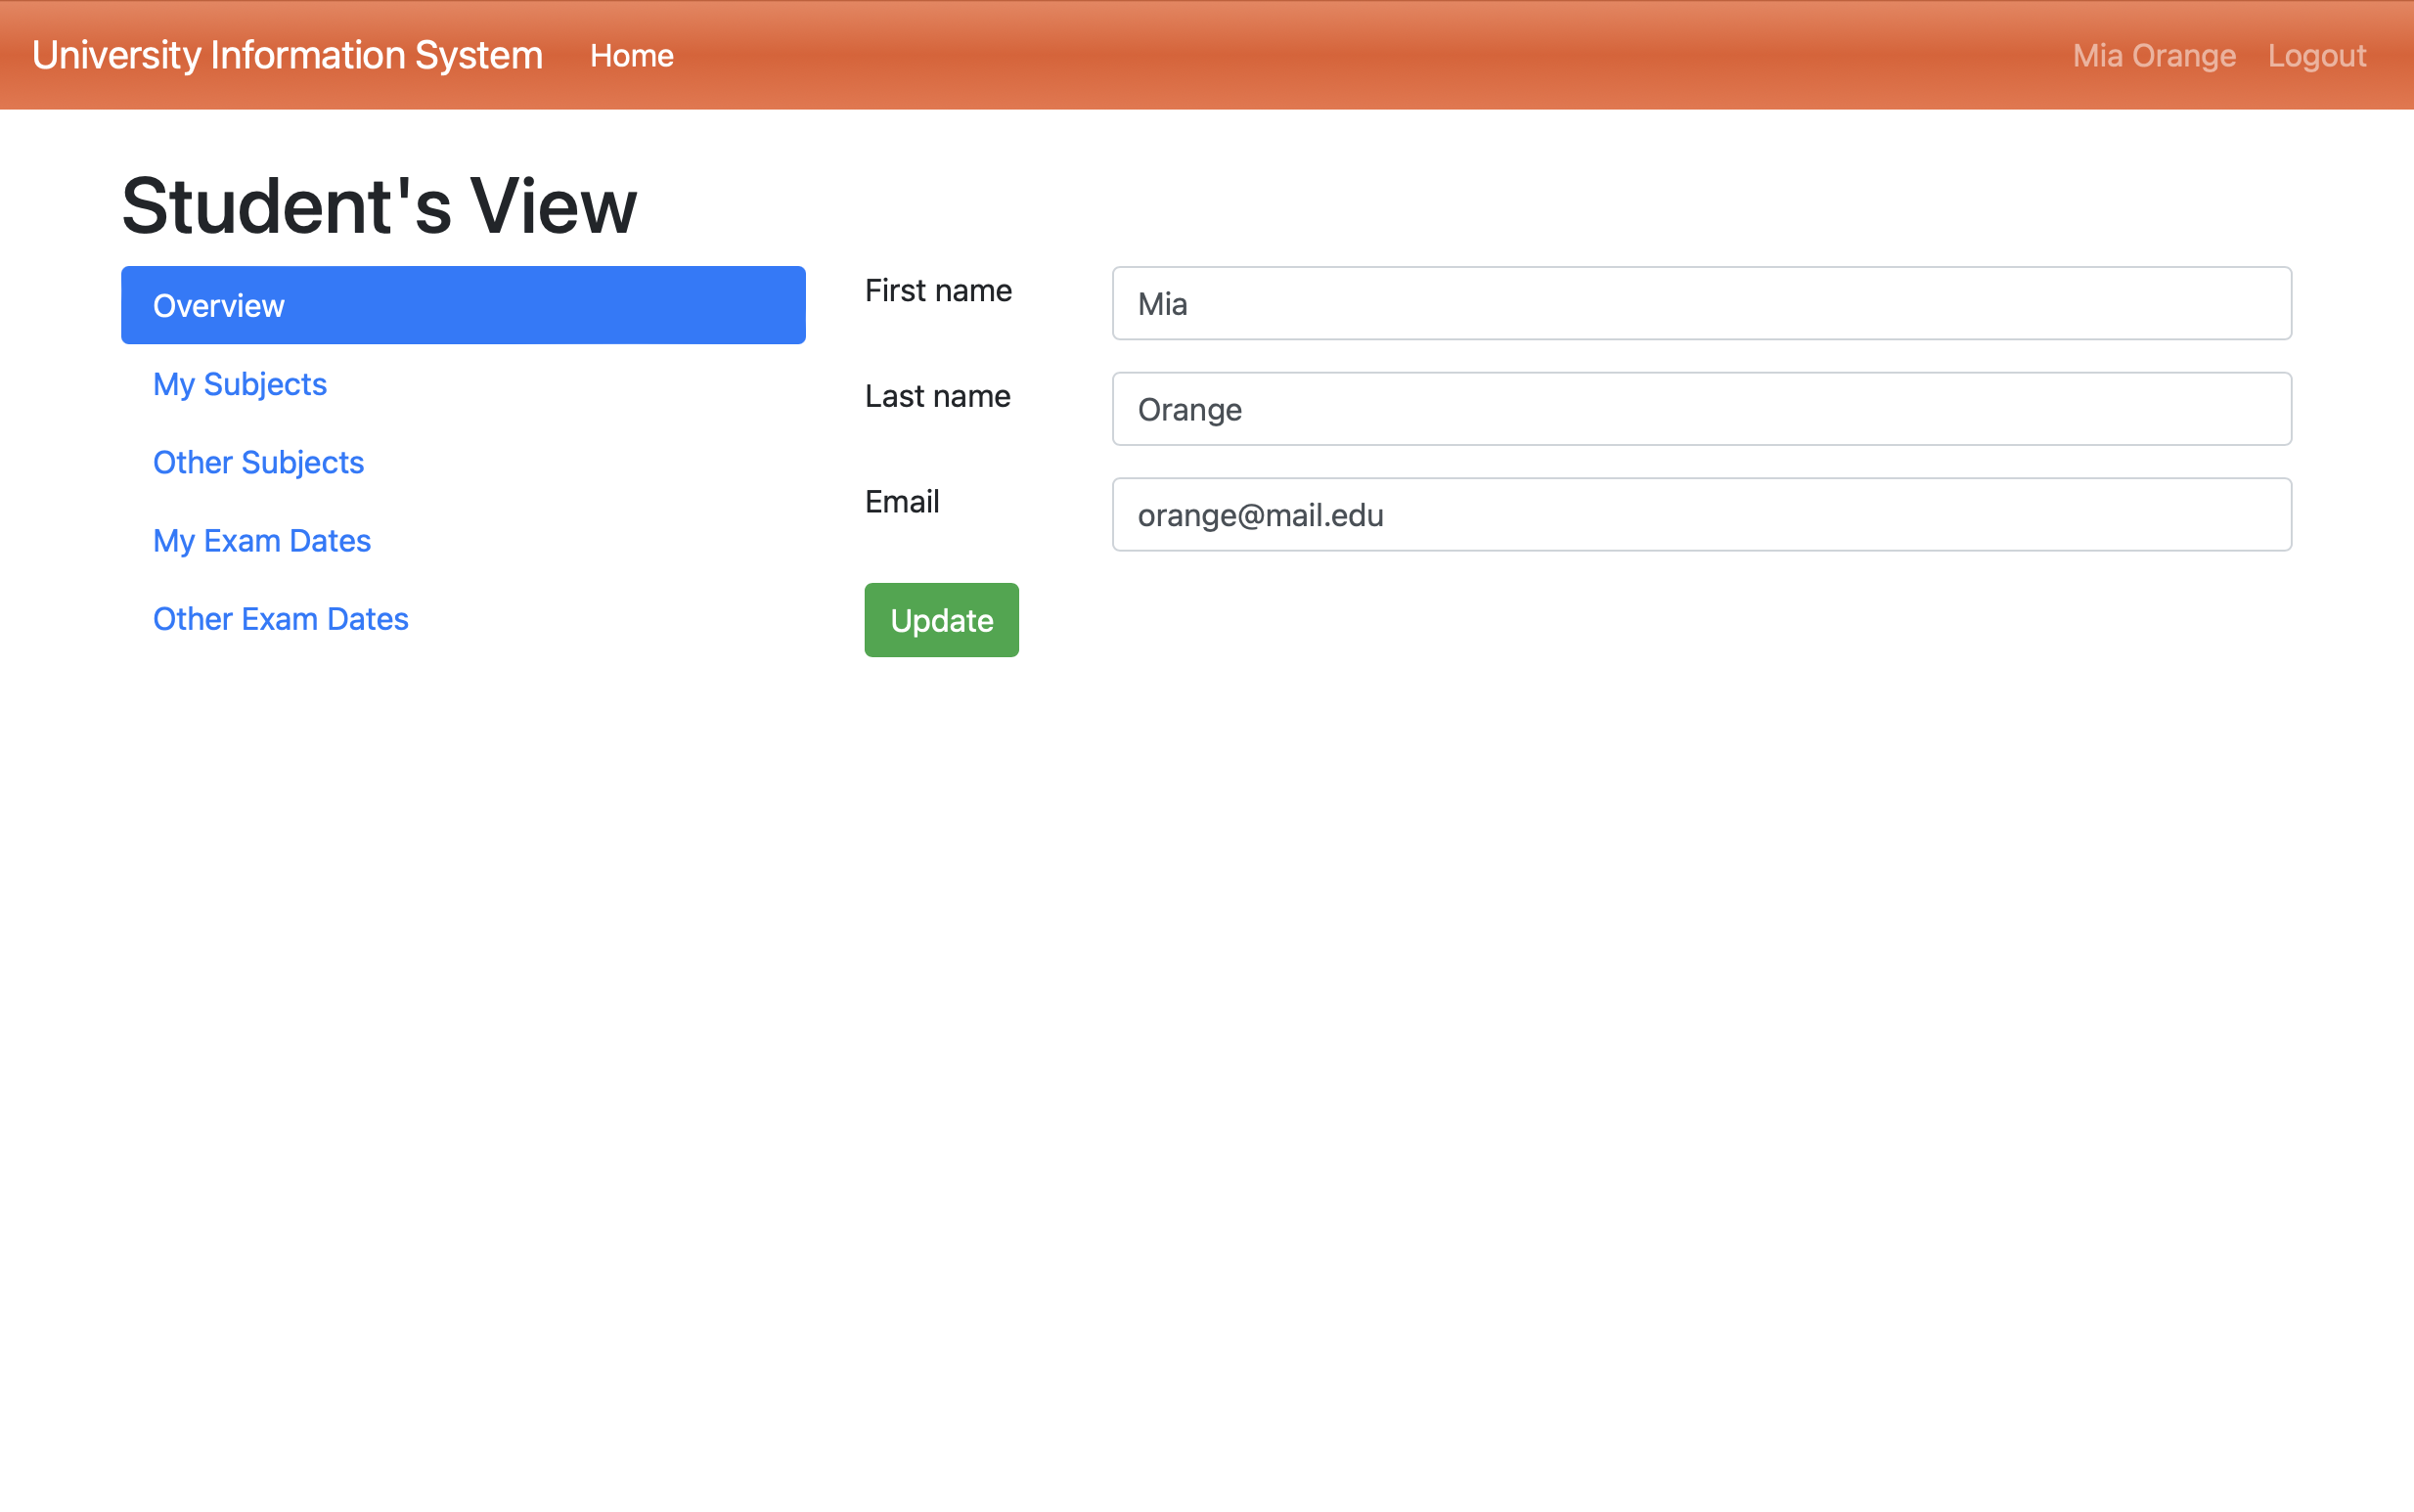
\includegraphics[width=0.8\textwidth]{pic/tbuis.png}
        \centering
        \caption{Prostředí systému TbUIS z pohledu studenta.}
        \label{fig:tbuis}
    \end{figure}

\chapter{Generování testů}

    \section{Výběr scénářů}

    Pro vygenerování testů za pomocí LLM bylo nejdříve nutné vybrat ze sady \textit{use caseů}\footnote{Seznam dostupný na adrese: \url{https://projects.kiv.zcu.cz/tbuis/web/page/uis#use-cases}} scénáře vhodné pro demonstraci nejen správné funkčnosti, ale také s možností ověření nesprávného chování na poruchových klonech (diskutováno v sekci \ref{sec:test_program}). Požadavek tedy byl, aby většina z vybraných scénářů vycházející z \textit{use casu} měl alespoň jeden poruchový klon, případně více. Vybráno bylo \(10\) scénářů, testovaných celkově na \(14\) variantách programu. Seznam vytvořených specifikací pro automatické generování testů se nachází v tabulkách \ref{tab:specs_1} a \ref{tab:specs_2}. Scénáře budou dále také referovány jako \textit{specifikace}. Každá specifikace má \textit{číslo}, které odpovídá číslu \textit{use casu}, ze kterého vychází (např. specifikace \(04\) vychází z use casu \textit{UC.04}). Zde je nutné poznamenat, že ne všechny specifikace vychází pevně z jejich use casů, ale byli upravené tak, aby šli provést v jednom chodu bez nutných závislostí (\textit{jako například namísto podmínky přihlášeného uživatele se uživatel vždy musí na začátku či během testu přihlásit do systému}). Popis specifikací v tabulce je pouze orientační a pro bližší upřesnění jednotlivých kroků, které se mají provést referujte web projektu. V tomto seznamu se také u každé specifikace nachází výčet klonů, na kterých lze očekávat poruchu. Celkový seznam klonů, a kterých se budou všechny vytvořené testy spouštět lze nalézt v tabulce \ref{tab:clones}. Podobně jako v případě specifikací, čísla klonů odpovídají číslům, jak jsou uvedena na oficiálním webu\footnote{Seznam poruchových klonů společně s možností stažení: \url{https://projects.kiv.zcu.cz/tbuis/web/page/download}} projektu společně s vysvětlením jednolivých chyb varianty. Pro přehlednost jsme bezchybnou variantu označili číslem \(00\).

    \vfill

    \begin{table}
        \begin{tabular}{|c|p{7cm}|c|}
            \hline
            \textbf{Specifikace} & \textbf{Popis} & \textbf{Porucha na klonech} \\
            \hline
            \(1\) & \textit{Přihlášení do aplikace} \newline Student i učitel se přihlásí do aplikace přihlašovacími údaji, dostupnými v databázi systému. Dále se zkontroluje, zda systém pro účet s neexistujícím uživatelským jménem nebo neplatným heslem vypíše chybovou hlášku. &  \(02\) \\
            \hline
            \(4\) & \textit{Odepsání předmětu} \newline Student se přihlásí, odepíše předmět v patřičné sekci systému. Předmět by následně měl zmizet v ostatních sekcích a to jak v pohledu studenta tak učitele. & \(04, 19, 25, 26, 28\) \\
            \hline
            \(6\) & \textit{Zapsání předmětu} \newline Student se přihlásí, zapíše předmět v patřičné sekci, který se následně zobarazí i v ostatních částech systému. Z učitelského pohledu by se student měl zobrazit na seznamu studentů daného předmětu. & \(25, 26, 28\) \\
            \hline
            \(8\) & \textit{Registrace na zkoušku} \newline Student se přihlásí do systémů a zapíše se na jeden z možných zkouškových termínů. Tento termín by se měl přesunout mezi již zapsané termíny. V učitelském pohledu bude student na seznamu zapsaných na konkrétní zkoušku a také by mělo být možno studenta ohodnotit. & \(22, 25, 26, 28\) \\
            \hline
            \(9\) & \textit{Zobrazení spolužáků u zkoušky} \newline Student se přihlásí a u zkoušky si může rozkliknout seznam všech účastníků. & \(\) \\
            \hline
            \(10\) & \textit{Zrušení předmětu} \newline Učitel po přihlášení klikne na tlačítko \textit{Remove} u předmětu, od jehož výuky se chce odhlásit. Ten se přestane zobrazovat ve všech ostatních sekcích systému z jeho pohledu, až na jeho znovuzapsání. Student by u předmětu neměl najít jméno daného učitele, který se odhlásil. & \(26, 28\) \\
            \hline
            \(11\) & \textit{Zobrazení studentů u předmětu} \newline Učitel se přihlásí do systému a u předmětu je schopen si zobrazit seznam zapsaných studentů. & \(26, 28\) \\
            \hline
        \end{tabular}
        \centering
        \label{tab:specs_1}
        \caption{Specifikace pro generované testy - část 1}
    \end{table}

    \begin{table}
        \begin{tabular}{|c|p{7cm}|c|}
            \hline
            \textbf{Specifikace} & \textbf{Popis} & \textbf{Porucha na klonech} \\
            \hline
            \(12\) & \textit{Zrušení zkoušky} \newline Učitel se přihlásí a v sekci jeho přidělených zkoušek odstraní konkrétní termín. Tento termín by nyní neměl být vidět jak v učitelském tak studentském pohledu do systému. & \(20, 21, 23, 26, 28\) \\
            \hline
            \(17\) & \textit{Přihlášení se k výuce předmětu} \newline Učitel se přihlásí do systému a v seznamu předmětů se přihlásí k výuce daného předmětu. Ten by se poté měl zobrazit ve zbytku systému v rámci patřičných sekcí. Zároveň studenti by nyní měli u předmětu vidět jméno tohoto vyučujícího. & \(18, 24, 25, 26, 27, 28\) \\
            \hline
            \(18\) & \textit{Zobrazení seznamu učitelů a předmětů, které vyučují} \newline Přihlášený učitel je schopen si zobrazit seznam všeech učitelů. & \(27, 28\) \\
            \hline
        \end{tabular}
        \centering
        \label{tab:specs_2}
        \caption{Specifikace pro generované testy - část 2}
    \end{table}

    \begin{table}
        \begin{tabular}{|c|c|}
            \hline
            \textbf{Číslo klonu} & \textbf{Porucha} \\
            \hline
            \(00\) & Bez defektu \\
            \hline
            \(02\) & Překlep v nadpisu \\
            \hline
            \(04\) & Návrat na špatnou stránkau\\
            \hline
            \(18\) & Chybějící sloupec v tabulce \\
            \hline
            \(19\) & Náhodně chybějící tlačítko \\
            \hline
            \(20\) & Nefunkční tlačítko \\
            \hline
            \(21\) & Změna se nepropíše do UI \\
            \hline
            \(22\) & Nefunkční tlačítko \\
            \hline
            \(23\) & Smazání se nepropíše do DB \\
            \hline
            \(24\) & Přidání se nepropíše do DB \\
            \hline
            \(25\) & Tabulka studentů prázdná \\
            \hline
            \(26\) & Tabulka učitelů prázdná \\
            \hline
            \(27\) & Nesprávný výběr z DB \\
            \hline
            \(28\) & Mix chyb (včetně interní chyby systému) \\
            \hline
        \end{tabular}
        \centering
        \label{tab:clones}
        \caption{Seznam poruchových klonů využitých pro testování.}
    \end{table}

    \section{Nahrávání scénářů}

    \section{Výběr požadavků}

    \section{Dotazování LLM}

        \subsection{Prostředí pro spuštění}

        \subsection{Dotazy}

\chapter{Spuštění testů}

    \section{Spuštění testovacího programu a jeho orchestrace}

\chapter{Vyhodnocení výsledků}

\chapter{Závěr}

% _____________________________________________________________________________
%
%
%        BACK MATTER (BIBLIOGRAPHY, LISTS, ...)
%
% _____________________________________________________________________________
%
\backmatter
\printbibliography
\listoffigures
\listoftables
\listoflistings
% _____________________________________________________________________________
%
%		BACK COVER
% _____________________________________________________________________________
%
%\setbackpagepic{img/fav} % <== an example of one possible option (read this manual)
%\setqrcodebaseurl{https://mycloud.org/show=pdf&docid=} % <== another example
%\setbackpageqrcode{54321} % <== and one more (uncomment the one that makes sense for you)
\setbackpageqrcode
\backpage
\end{document}
